% !TEX root = lectnote.tex
% !TEX spellcheck = en_GB-oed 

\chapter{Counting}\label{cha:counting}


In this Chapter we will consider counting problems. 
These will be problems, 
where we need to count the number of possibilities of something happening. 
Let us warm up to this first by solving some easy exercises. 

At the ``Freshmen's party'' several people meet. 
Five friends (Arnold, Bill, Carl, David, Edmund) greet each other at this party by shaking hands. 
How many handshakes does this mean? 
It is not too hard to count all possibilities: 
Arnold shakes hand with Bill, Carl, David, Edmund, 
Bill shakes hand with Carl, David, Edmund (we have already counted the Arnold-Bill handshake), 
Carl shakes hand with David and Edmund (we have already counted the Arnold-Carl and Bill-Carl handshake), 
David shakes hand with Edmund (we have already counted all other handshakes with David), 
and all handshakes with Edmund is already accounted for. 
That is, there are $4 + 3 + 2 + 1 = 10$ handshakes altogether. 

Now, this was easy, but this party is very big, and a lot of people attend it. 
Say, there are 200 College freshmen greeting each other by shaking hands. 
How many handshakes are there? 
We can try to generalize our former argument. 
Let us count the number of handshakes by ordering the people in some way 
(say, by date of birth). 
That is, first we count the handshakes by the oldest person, 
then the handshakes by the second oldest person, etc. 
The oldest person shakes hand with 199 other people, 
this is 199 handshakes. 
The second oldest person shakes hand with 199 people, as well, 
but we have already counted 1 handshake with the oldest person. 
That is, we count 198 more handshakes. 
For the third oldest person, out of 199 handshakes we have already counted 2: 
one with the oldest person and one with the second oldest person. 
That is, we count 197 more handshakes, etc. 
Continuing this argument, 
we count one less handshakes with each person. 
For the second youngest people we count only one new handshake: the handshake with the youngest person. 
And finally, for the youngest person we have already counted all handshakes. 
That is, the number of handshakes is 
\[
199 + 198 + 197 + \dots + 1. 
\]
How much is this number? 
Is there an easier way to calculate it, 
rather than adding all these numbers together? 
Those who are familiar with arithmetic progressions can calculate easily that the answer is $\frac{199 \cdot 200}{2} = 19~900$. 
But even without that knowledge, 
we can calculate this sum by observing that the sum of the first and last number is 200. 
Then the sum of the second and one but last number is 200, again. 
We can continue this argument, and reach $99+101=200$, 
and the number 100 is left alone. 
That is, 
\begin{align*}
& 1 + 2 + \dots + 198 + 199 = (1 + 199) + (2 + 198) + \dots + (99 + 101) + 100 \\
& = 99\cdot 200 + 100 = (99 \cdot 2 + 1 ) \cdot 100 = 19~900. 
\end{align*}

This summation argument works in general, as well: 

\begin{proposition}\label{prop:sumk}
For a positive integer $n$ we have 
\[
1 + 2 + \dots + (n-1) + n = \frac{n \cdot (n+1)}{2}. 
\]
\end{proposition}

\begin{exercise}\label{ex:sumk}
Prove Proposition~\ref{prop:sumk} by using the argument described above. 
Make two cases depending on whether $n$ is even or odd. 
\end{exercise}

\begin{proof}
We show another proof here, 
which is usually attributed to Carl Friedrich Gauss.\footnote{German mathematician and physicist, 1777--1855.} 
Let $S$ be the sum of the integers from 1 to $n$, 
and write the same sum in reverse order below: 
\begin{align*}
S &= 1 + 2 + \dots + (n-1) + n, \\
S &= n + (n-1) + \dots + 2 + 1. 
\intertext{Adding the two equations together, we obtain}
2S &= (1+n) + (2 + n-1) + \dots + (n-1 + 2) + (n+1), \\
2S &= (n+1) + (n+1) + \dots + (n+1) + (n+1),\\
2S &= n \cdot (n+1), \\
S &= \frac{n\cdot (n+1)}{2}. 
\end{align*}
\end{proof}

Now, we are able to tell the number of handshakes between $n$ people. 
Using the same line of thought, 
the first person shakes hand with $(n-1)$ other people, 
the next one with $(n-2)$ other people (we already counted the handshake with the first person), etc. 
That is, the number of handshakes between $n$ people is 
\[
(n-1) + (n-2) + \dots + 1, 
\]
which is $\frac{(n-1)\cdot n}{2}$ by Proposition~\ref{prop:sumk} (writing $(n-1)$ instead of $n$). 
Thus, we have proved

\begin{corollary}\label{cor:handshakes}
The number of handshakes between $n$ people is 
\[
1 + 2 + \dots + (n-1) = \frac{(n-1)\cdot n}{2}. 
\]
\end{corollary}

\begin{proof}
Even though we have already proved the statement above, 
we give here an alternative proof. 
The reason for this is that this proof method will be useful later on. 

Every person shakes hand with $(n-1)$ other people. 
Altogether there are $n$ people, 
this would mean $(n-1) \cdot n$ handshakes. 
But this way every handshake is calculated twice: 
a handshake between $A$ and $B$ is calculated once for $A$ and once for $B$. 
Thus, in reality, $(n-1) \cdot n$ is twice the number of handshakes. 
That is, the number of handshakes is $\frac{(n-1) \cdot n}{2}$. 
\end{proof}

\begin{exercise}\label{ex:5people3hanshake}
Five friends meet at this party. 
Some of them shake hands. 
Is it possible that everyone shook hands exactly three times? 
What is the answer if a person can shake hands with another more than once? 
What are the answers if seven people meet? 
\end{exercise}

Four girls (Alice, Beth, Carrie, Diane) 
and four boys (Ed, Frank, George, Hugo) meet at this party. 
As a greeting any two boys shake hands with each other, 
but with the girls the two parties kiss each other on the cheek. 
\begin{exercise}\label{ex:kisses}
How many handshakes and kisses are there? 
\end{exercise}
After greeting each other, 
they want to dance. 
In fact, every boy wants to dance with every girl, 
and they are interested in how many rounds they need to achieve this. 

First, 
let us count the number of ways they can form dancing couples (one boy and one girl). 
There are four boys, and four girls, every boy wants to dance with every girl, 
that is, there are altogether $4 \cdot 4 = 16$ possible couples. 
We can even list these 16 possibilities: 

%\medskip
\vskip 12pt
\begin{tabular}{llll}
Alice -- Ed & Beth -- Ed & Carrie -- Ed & Diane -- Ed \\
Alice -- Frank & Beth -- Frank & Carrie -- Frank & Diane -- Frank \\
Alice -- George & Beth -- George & Carrie -- George & Diane -- George \\
Alice -- Hugo & Beth -- Hugo & Carrie -- Hugo & Diane -- Hugo 
\end{tabular}
%\medskip
\vskip 12pt

In one round four couples can dance. 
How many ways can they form four dancing couples for one round? 
Assume that each girl chooses a partner in a certain order. 
First Alice chooses a partner, then Beth, then Carrie, and finally Diane dances with whoever is left. 
Alice has four choices, because she can choose any of the boys. 
Beth will only have three choices, because Alice will have already chosen someone. 
Carrie will have only two choices, because Alice and Beth will have already chosen someone. 
Finally, Diane has only one choice. 
Altogether, they have $4 \cdot 3 \cdot 2 \cdot 1 = 24$ possibilities to form four dancing couples at the same time. 

%\begin{exercise}
%Why do we multiply these numbers instead of adding them together? 
%\end{exercise}
%
%\begin{exercise}
%Would we have arrived at a different answer if Diane has the first choice? 
%\end{exercise}

Now, in one round at most four couples can dance. 
Therefore they will need at least $\frac{16}{4} = 4$ rounds for everyone dancing with everyone else. 
But be careful! 
We only proved that they need 4 rounds, 
we have not proved that they can actually do it in 4 rounds. 
The easiest is to just give a ``schedule'' for the 16 couples in each rounds, e.g.\ see Table~\ref{tab:dancing}
\begin{table}[!htbp]
\caption{Four couples dancing in four rounds}\label{tab:dancing}
\begin{center}
\begin{tabular}{llll}
1st round & 2nd round & 3rd round & 4th round \\
\hline
Alice -- Ed & Beth -- Ed & Carrie -- Ed & Diane -- Ed \\
Beth -- Frank & Alice -- Frank & Diane -- Frank & Carrie -- Frank \\
Carrie -- George & Diane -- George & Alice -- George & Beth -- George \\
Diane -- Hugo & Carrie -- Hugo & Beth -- Hugo & Alice -- Hugo 
\end{tabular}
\end{center}
\end{table}
\vfill\eject
% How many ways can we fill out this table? 
% It is $6\cdot 2$ for 3 couples. 
% It is $24 \cdot 9 \cdot (1+1)$ for 4 couples.  

\begin{exercise}\label{ex:isitpossible1}
Is it possible
\begin{enumerate}
\item[(a)] 
to distribute 100 rabbits into five packs such that each pack contains an odd number of rabbits? 
\item[(b)] 
that both the sum and the product of some integer numbers are 9? 
\item[(c)] 
that both the sum and the product of 9 integer numbers are 9? 
\item[(d)] 
that the sum of 9 integer numbers is 0 and the product of these numbers is 9? 
\end{enumerate}
\end{exercise}

\begin{exercise}\label{ex:sum24}
\begin{enumerate}
\item[(a)] What is the sum of the first 24 positive integers, i.e.\ $1 + 2 + 3 + \dots + 23 + 24 = $?
\item[(b)] Compute $\frac{1 + 2 + 3 + 4 + \dots + 23 + 24}{1 - 2 + 3 - 4 +  \dots + 23 - 24}$. 
\end{enumerate}
\end{exercise}

%\begin{exercise}\label{ex:wedding}
%Five girls and seven boys play wedding (three of the girls have one brother, each). 
%They choose (in the following order) the wedding couple, a registrar, two bridesmaids, 
%two boys for accompanying the bridesmaids, and two witnesses. 
%There are some rules, though: 
%the wedding couple cannot be brother and sister, 
%and the registrar cannot be a sibling of anyone of the wedding couple. 
%\begin{enumerate}
%\renewcommand{\theenumi}{(\alph{enumi})}
%% This is not exactly what I want, because I would not have the dot at the end. 
%% That would need the enumerate environment. 
%\item 
%How many ways can they choose the people for the wedding? 
%\item 
%Do we arrive at the same answer if the registrar is chosen at the end rather than right after the wedding couple? 
%\end{enumerate}
%\end{exercise}




\section{Sequences}\label{sec:sequences}

In Section~\ref{sec:numeralsystem} we have learned how to write a number in different numeral systems. 
We are now interested in how many $n$-digit numbers exist in a certain numeral system. 
Let us start with base 10. 
We know that there are 9 one-digit positive integers: 1, 2, 3, 4, 5, 6, 7, 8, 9. 
How many two digit positive integers exist? 
One way to count them is that we know that there are 99 positive integers which are one-digit or two-digit long. 
We have already counted that there are 9 one-digit positive integers. 
Therefore there are $99-9=90$ two-digit positive integers. 

We could have calculated this differently: 
there are 9 possibilities for a first digit of a two-digit number, 
and there are 10 possibilities (independently from the first digit) for the second digit. 
That is, there are $9 \cdot 10$ two-digit positive integers. 

Now, what about three-digit positive integers? 
There are 999 `at most three-digit numbers', 
and 99 are `at most two-digit numbers'. 
Thus there are $999-99=900$ three-digit positive integers. 
But we can obtain this result by using the other idea, as well. 
There are 9 possibilities for the first digit of a three-digit number, 
10 possibilities for the second digit and 10 possibilities for the third digit, 
that makes $9 \cdot 10 \cdot 10 = 900$ possibilities for three digit positive integers. 

Let us generalize this argument for $n$-digit positive integers. 
There are 9 possibilities for the first digit, 
and 10 possibilities for every other digit. 
Altogether, the number of $n$-digit positive integers (in base 10) is
\[
9 \cdot \underbrace{10 \cdot \dots \cdot 10}_{n-1} = 9\cdot 10^{n-1}. 
\]

\begin{exercise}\label{ex:noofbase2numbers}
How many $n$-digit base 2 positive integers exist? 
\end{exercise}

We could generalize this idea for arbitrary bases. 

\begin{proposition}\label{prop:numberofndigitbasek}
The number of $n$-digit base $k$ positive integers is 
\[
(k-1) \cdot k^{n-1}.
\] 
\end{proposition}

\begin{proof}
There are $(k-1)$-many possibilities for the first digit (it cannot be 0, only $1, 2, \dots, k-1$), 
and there are $k$ possibilities for every other digit. 
Thus, the number of $n$-digit positive integers in base $k$ is
\[
(k-1) \cdot \underbrace{k \cdot \dots \cdot k}_{n-1} = (k-1) \cdot k^{n-1}. 
\]
\end{proof}

And what about the ``at most'' $n$-digit non-negative integers in base $k$ (including 0)? 
In this case, we can consider them as $n$-digit numbers, 
where the first digit can be 0, as well. 
Thus, there are $k$ possibilities for the first digit, 
$k$ possibilities for the second digit, etc. 
Thus, 
\begin{proposition}\label{prop:numberofnatmostdigitbasek}
The number of ``at most'' $n$-digit non-negative integers in base $k$ is
\[
\underbrace{k \cdot k \cdot \dots \cdot k}_{n} = k^n. 
\]
\end{proposition}

In a very similar way we can count the number of possible 5 letter long words. 
(Here, we count the not necessarily meaningful words, as well.)
Indeed, 
as the English alphabet consists of 26 letters, 
we have 26 possibilities for the first letter, 
26 possibilities for the second letter, etc. 
That is, 
the number of 5 letter long words is 
\[
26 \cdot 26 \cdot 26 \cdot 26 \cdot 26 = 26^5. 
\]

It seems, that it is easy to calculate sequences of letters (i.e.\ possible words), 
as long as we know how long they should be and how many letters the alphabet has. 
Indeed, we can formulate our main theorem. 

\begin{theorem}\label{thm:sequence}
Let the alphabet consist of $k$ letters. 
Then the number of $n$ letter long sequences (possible words) is $k^n$. 
\end{theorem}

\begin{proof}
There are $k$ possibilities to choose the first letter. 
Then, there are $k$ possibilities to choose the second letter (no matter how we have chosen the first letter), etc. 
Altogether there are $n$ letters to choose (with possible repetitions), 
thus the number of $n$ letter long sequences is 
\[
\underbrace{k \cdot k \cdot \dots \cdot k}_{n} = k^n. 
\]
\end{proof}

Sometimes this theorem needs to be combined for different alphabets for each letter. 
We already saw an example: 
for calculating the number of $n$-digit long base 10 numbers, 
the first digit is an element of an alphabet of size 9, 
and every other $(n-1)$ digit can be an element of size 10. 
As the choice of the digits is independent to each other, 
the number of $n$-digit base 10 numbers is $9 \cdot 10^{n-1}$. 

Another possible example is the mobile phone number of a person. 
In Hungary, there are three mobile providers, 
and each provider issues 7 digit long numbers. 
Thus altogether there are $3 \cdot 10^7$ possibilities for a mobile phone number in Hungary. 

\begin{exercise}\label{ex:palindrome}
How many 3 digit palindrome numbers exist (in base 10)? 
(Palindrome numbers are numbers which are the same if read backwards. 
How many at most 3 digit palindrome numbers exist (in base 10)? 
Generalize the result to $n$-digit base $k$ palindrome numbers. 
\end{exercise}

\begin{exercise}\label{ex:Hungarianwords}
The Hungarian alphabet contains 44 letters. 
How many 5, 7, 10 letter long (not necessarily meaningful) words can be created using Hungarian letters? 
\end{exercise}

\begin{exercise}\label{ex:toto}
In Hungary there is a game called ``TOTÓ'', 
where one bets on the outcome of certain football games. 
There are $13+1$ games one can bet on, 
and there are 3 choices for each of them: 
one writes `1' if they think that the first team wins, 
one writes `2' if they think that the second team wins, 
and `X' means that the result is a draw. 
How many TOTÓ tickets should be filled out to make sure that one of them will be correct for all $13+1$ games? 
\end{exercise}

\begin{exercise}\label{ex:company}
In a company the following system is used to record the people working there: 
in the first record the name of the person is written as a 20 long string with possible spaces. 
Then the gender of the person is put into the next record (male/female). 
Then follows the person's job title in a 10 letter long string, 
and finally comes the payment of the person as an at most 8 digit non-negative integer in base 10. 
How many people records can be stored in this system if we allow empty names/job titles, as well? 
\end{exercise}





\section{Number of subsets}\label{sec:subsets}

In Section~\ref{sec:sets} we have learned what a set is, 
and what its subsets are. 
Now, we want to count these subsets. 
Let us begin with some exercises. 

\begin{exercise}\label{ex:subsetsof3elemetset}
List all subsets of %the sets 
$\halmaz{1, 2, 3}$, $\halmaz{a, b, c}$, $\halmaz{\text{Alice, Beth, Carrie}}$, $\halmaz{\text{apple, banana, cherry}}$. 
How many subsets do these sets have? 
\end{exercise}

After solving Exercise~\ref{ex:subsetsof3elemetset}, 
one suspects that the number of subsets depend only on the cardinality of the set, 
and not on the actual elements of the set. 
This is true in general: 
for example if a set has three elements, 
then we might as well name the elements $a$, $b$ and $c$, 
and then its subsets will be exactly the same as we determined in Exercise~\ref{ex:subsetsof3elemetset}. 

Let us try to determine the number of subsets of a set with given cardinality. 
Let $S$ be a set of cardinality 0, i.e.\ $S = \emptyset$. 
Then $S$ has only one subset: $\emptyset$. 
If $S$ is a set of cardinality 1, e.g.\ $S = \halmaz{a}$, 
then it has two subsets: $\halmaz{} = \emptyset$, $\halmaz{a} = S$. 
If $S$ is a set of cardinality 2, e.g.\ $S = \halmaz{a, b}$, 
then it has four subsets: $\halmaz{} = \emptyset$, $\halmaz{a}$, $\halmaz{b}$, $\halmaz{a, b} = S$. 
If $S$ is a set of cardinality 3, e.g.\ $S = \halmaz{a, b, c}$, 
then it has eight subsets: $\halmaz{} = \emptyset$, $\halmaz{a}$, $\halmaz{b}$, $\halmaz{c}$, 
$\halmaz{a, b}$, $\halmaz{a, c}$, $\halmaz{b, c}$, 
$\halmaz{a, b, c} = S$. 
Figure~\ref{fig:subsetsabc} shows all subsets of $\halmaz{a, b, c}$. 
In this figure, two sets are connected if the lower one is a subset of the upper one. 
Table~\ref{tab:noofsubsets} summarizes our findings on the number of subsets so far. 

\begin{figure}[!htb]
\begin{center}
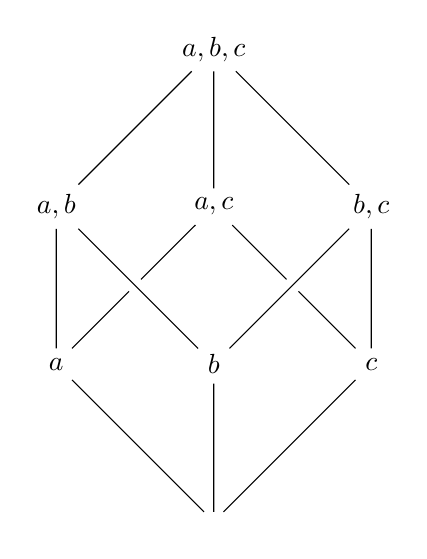
\begin{tikzpicture}
  \node (max) at (0,4) {$\halmaz{a, b, c}$};
  \node (a) at (-2,2) {$\halmaz{a, b}$};
  \node (b) at (0,2) {$\halmaz{a, c}$};
  \node (c) at (2,2) {$\halmaz{b, c}$};
  \node (d) at (-2,0) {$\halmaz{a}$};
  \node (e) at (0,0) {$\halmaz{b}$};
  \node (f) at (2,0) {$\halmaz{c}$};
  \node (min) at (0,-2) {$\halmaz{}$};
  \draw (min) -- (d) -- (a) -- (max) -- (b) -- (f)
  (e) -- (min) -- (f) -- (c) -- (max)
  (d) -- (b);
  \draw[preaction={draw=white, -,line width=6pt}] (a) -- (e) -- (c);
\end{tikzpicture}
\end{center}
\caption{Subsets of $\halmaz{a, b, c}$.}\label{fig:subsetsabc}
\end{figure}

\begin{table}[!htb]
\caption{Number of subsets}\label{tab:noofsubsets}
\begin{center}
\begin{tabular}{|c|c|}
\hline
Cardinality of $S$ & Number of subsets of $S$ \\
\hline \hline
$0$ & $1$ \\
\hline
$1$ & $2$ \\
\hline
$2$ & $4$ \\
\hline
$3$ & $8$ \\
\hline
\end{tabular}
\end{center}
\end{table}

\begin{exercise}\label{ex:abcde}
Guess what the rule is by looking at Table~\ref{tab:noofsubsets} and listing all subsets of $\halmaz{a, b, c, d}$ and $\halmaz{a, b, c, d, e}$, if necessary. 
\end{exercise}

It seems that if $S$ has $n$ elements, 
then it has $2^n$ subsets. 
This is reinforced by Figure~\ref{fig:subsetsabc}, 
where we represented the subsets of a three-element set by the eight vertices of a cube. 
This conjecture is true in general: 

\begin{theorem}\label{thm:noofsubsets}
Let $S$ be a set of cardinality $n$ for some $n\geq 0$ integer. 
Then $S$ has $2^n$-many subsets. 
\end{theorem}

\begin{proof}
Let us denote the elements of $S$ by $a_1, a_2, \dots , a_n$, 
that is, 
\[
S = \halmaz{a_1, a_2, \dots , a_n}. 
\]
Let us try to build a subset $T$ of $S$, 
and we count the number of possibilities to create different subsets $T$. 
First we decide whether or not $a_1 \in T$, 
that is, whether or not we put $a_1$ into $T$. 
This gives us two choices. 
Now, independent of how we decided on $a_1$, 
we decide whether or not we want to put $a_2$ into $T$, 
that is, whether or not $a_2 \in T$. 
This, again, gives us two choices. 
Third (independently on how we decided on the earlier elements)
we decide whether or not we put $a_3$ into $T$, 
that is, whether or not $a_3 \in T$. 
This, again, gives us two choices, etc. 

This way we decide after each other for every element whether or not we want to put the element into $T$. 
On the one hand, 
if at some point we choose differently, then we obtain different subsets in the end. 
For example, if for $a_k$ we decide differently, 
then in one case $a_k$ will be an element of the subset, 
in the other case it will not be an element. 
Thus the two subsets will differ in $a_k$. 
On the other hand, 
all subsets can be obtained this way: 
for a subset $A$ we decide to put the elements of $A$ into $T$, 
and not put other elements in. 
This way, $T=A$ will be built. 

That is, by deciding for every element whether or not it should be in $T$ we obtain all subsets exactly once. 
For each element we have two choices: 
either we put them into the subset or we do not put them into the subset. 
These choices on the elements are independent from each other, 
thus for all $n$ elements we have 
\[
\underbrace{2 \cdot 2 \cdot \dots \cdot 2}_{n} = 2^n
\]
choices. 
This is the same as the number of subsets of $S$. 
Thus an $n$ element set has $2^n$-many subsets. 
\end{proof}

\begin{exercise}\label{ex:subsettrytheproof}
For $S= \halmaz{a, b, c}$ obtain all subsets using this decision algorithm. 
\end{exercise}

There are different ways to obtain the same result. 
Another argument can be the following:

\begin{proof}[Second proof of Theorem~\ref{thm:noofsubsets}]
We give a draft of the proof, which can be made precise after reading about mathematical induction. 
Again, let us denote the elements of $S$ by $a_1, a_2, \dots , a_n$, 
that is, 
\[
S = \halmaz{a_1, a_2, \dots , a_n}. 
\]
Here, every subset either contains $a_n$ or does not contain $a_n$. 

First, consider those subsets, which do not contain $a_n$, 
and let $S' = \halmaz{a_1, a_2, \dots, a_{n-1}}$. 
Observe that a subset of $S$ not containing $a_n$ is in fact a subset of $S'$. 
Moreover, every subset of $S'$ is a subset of $S$ not containing $a_n$. 
That is, there is a one-to-one correspondence between the subsets of $S$ not containing $a_n$ and the subsets of $S'$. 

Now, consider the subsets of $S$ containing $a_n$. 
Observe that a subset of $S$ containing $a_n$ is in fact a union of a subset of $S'$ and $\halmaz{a_n}$. 
That is, it is $a_n$ added to a subset of $S'$. 
Moreover, if we add $a_n$ to every subset of $S'$ we obtain a subset of $S$ containing $a_n$. 
That is, there is a one-to-one correspondence between the subsets of $S$ containing $a_n$ and the subsets of $S'$. 

Thus, the number of subsets of $S$ is twice as the number of subsets of $S'$. 
Continuing this argument, 
we obtain that the number of subsets of $S$ is 4 times the number of subsets of $\halmaz{a_1, \dots , a_{n-2}}$, etc. 
That is, the number of subsets of $S$ is $2^n$ times the number of subsets of $\halmaz{} = \emptyset$. 
As the latter has only 1 subset, $S$ has exactly $2^n$-many subsets. 
\end{proof}

Note, that this argument would not have been necessary, 
as we have already proved the statement of Theorem~\ref{thm:noofsubsets}. 
Therefore this new proof does not make the statement any more true 
(in any case, a mathematical statement is either true or not true, there are no degrees to how true it is). 
What it provides is a different insight into how we can build subsets of a set. 
For example, this argument can be useful if we need certain types of subsets: 

\begin{exercise}\label{ex:subsetabcd}
List all subsets of $S = \halmaz{a, b, c, d}$ not containing $d$, 
and note that they are exactly the subsets of $\halmaz{a, b, c}$. 
Then list all subsets of $S = \halmaz{a, b, c, d}$ containing $d$, 
and note that they are exactly the subsets of $\halmaz{a, b, c}$ with $d$ added to them. 
\end{exercise}

It is an interesting coincidence that there are $2^n$ subsets of an $n$-element set, 
and that exactly $2^n$-many at most $n$-digit binary numbers exist. 
Such a coincidence always makes a mathematician suspicious 
that there might be more to it than just accidental equality. 

\begin{exercise}\label{ex:subsetabcd01}
Encode all subsets of $S = \halmaz{a, b, c, d}$ in the following way: 
for every subset $T$ we assign an at most four digit binary number. 
The first digit is 0 if $d \notin T$, and 1 if $d \in T$. 
Similarly, the second digit is 0 if $c \notin T$, and 1 if $c \in T$. 
The third digit is 0 if $b \notin T$, and 1 if $b \in T$. 
Finally, the fourth digit is 0 if $a \notin T$, and 1 if $a \in T$. 
Note that this is a one-to-one correspondence between the subsets and the at most four digit binary numbers. 
\end{exercise}

The idea of Exercise~\ref{ex:subsetabcd01} works in general, as well: 

\begin{proof}[Third proof of Theorem~\ref{thm:noofsubsets}]
This time it is probably more helpful to denote the elements of $S$ by $a_0, a_1, \dots , a_{n-1}$, 
that is, 
\[
S = \halmaz{a_0, a_1, \dots , a_{n-1}}. 
\]
Now, we assign an at most $n$-digit binary number to every subset of $S$. 
Let $T$ be an arbitrary subset of $S$, 
and we assign a binary number to it in the following way. 
Its last digit (corresponding to $2^0$) is 0 if $a_0 \notin T$ and 1 if $a_0 \in T$. 
Similarly, the one but last digit (corresponding to $2^1$) is 0 if $a_1 \notin T$ and 1 if $a_1 \in T$. 
In general, the $(k+1)$st digit from the back (corresponding to $2^k$, $0\leq k\leq n-2$) is 0 if $a_k \notin T$ and 1 if $a_k \in T$. 
Finally, the first digit (corresponding to $2^{n-1}$) is 0 if $a_{n-1} \notin T$ and 1 if $a_{n-1} \in T$. 
This way we assigned an at most $n$-digit binary number to every subset. 
For different subsets we assigned different binary numbers, 
and for every number we can easily generate the subset corresponding to it 
(we just need to add those elements into the subset where the digit is 1). 
That is, this encoding is a one-to-one correspondence between subsets of $S$ and the at most $n$-digit binary numbers. 
By Proposition~\ref{prop:numberofnatmostdigitbasek} we know that there are $2^n$-many at most $n$-digit binary numbers. 
Thus, $S$ has $2^n$-many subsets, as well. 
\end{proof}

This third proof, again, gives something extra to our knowledge. 
Now, we have enumerated all the subsets of $S$, 
and if we are interested in the $k$th subset, 
we can easily compute it. 

\begin{exercise}\label{ex:encode1}
Let $S = \halmaz{a_0, a_1, a_2, a_3}$. 
Let us encode the subsets of $S$ as in the third proof of Theorem~\ref{thm:noofsubsets}. 
Compute the subsets corresponding to the binary representation of $11$, $7$, $15$. 
\end{exercise}

\begin{exercise}\label{ex:encode2}
Let $S = \halmaz{a_0, a_1, a_2, a_3, a_4}$. 
Let us encode the subsets of $S$ as in the third proof of Theorem~\ref{thm:noofsubsets}. 
Compute the subsets corresponding to the binary representation of $11$, $7$, $15$, $16$, $31$. 
Compare the results to those of Exercise~\ref{ex:encode1}. 
\end{exercise}

\begin{exercise}\label{ex:encode3}
Let $S = \halmaz{a_0, a_1, a_2, a_3, a_4, a_5}$. 
Let us encode the subsets of $S$ as in the third proof of Theorem~\ref{thm:noofsubsets}. 
Compute the subset corresponding to the binary representation of $49$. 
\end{exercise}

\begin{exercise}\label{ex:encode4}
Let $S = \halmaz{a_0, a_1, a_2, a_3, a_4, a_5, a_6}$. 
Let us encode the subsets of $S$ as in the third proof of Theorem~\ref{thm:noofsubsets}. 
Compute the subset corresponding to the binary representation of $101$. 
\end{exercise}

\begin{exercise}\label{ex:encode5}
Let $S = \halmaz{a_0, a_1, a_2, a_3, a_4, a_5, a_6, a_7}$. 
Let us encode the subsets of $S$ as in the third proof of Theorem~\ref{thm:noofsubsets}. 
Compute the subset corresponding to the binary representation of $199$. 
\end{exercise}






\section{Permutations}\label{sec:permutations}

Three students are taking an oral exam in Mathematics. 
After the usual half hour preparation time, 
one by one they tell the examiner about the theorem the examiner gave them. 
In how many different order can they do the exam? 
Let the three students be Alice, Beth and Claire. 

It is not hard to list all possibilities. 
For example, Alice can start the exam, 
and then Beth follows and Claire finishes, 
or Claire follows and Beth finishes. 
Similarly, Beth can start with the exam, 
then Alice can follow and then Claire, 
or Claire and then Alice. 
Finally, 
Claire may start, and Alice continues and then Beth, 
or Beth continues and Alice finishes. 
Table~\ref{tab:perm1} lists all six possibilities. 

\begin{table}[!htb]
\caption{The orders in which Alice, Beth and Claire can take the exam}\label{tab:perm1}
\begin{center}
\begin{tabular}{c|c|c}
first & second & third \\
\hline
Alice & Beth & Claire \\
Alice & Claire & Beth \\
Beth & Alice & Claire \\
Beth & Claire & Alice \\
Claire & Alice & Beth \\
Claire & Beth & Alice
\end{tabular}
\end{center}
\end{table}

Looking at Table~\ref{tab:perm1}, 
one can think of a general argument, as well. 
There are three ways to choose who the first person will be (Alice, Beth or Carrie). 
Then no matter what that choice was, 
there will be two possibilities left for choosing who the second person will be 
(the second person cannot be whoever was the first one). 
Then the person left will take the exam as the third. 
Altogether, this is $3 \cdot 2 \cdot 1 = 6$ possibilities. 

At the next exam, 
there are four students: 
Ed, Frank, George, Hugo. 
This time they decide in advance in what order they want to do the exam. 
In how many different orders can they do the exam? 

\begin{exercise}\label{ex:ExamEFGH}
List all possibilities for Ed, Frank, George and Hugo to find an order for themselves. 
\end{exercise}

Let us try to use our new argument. 
There are four possibilities for choosing the person who starts the exam. 
Then, no matter who starts, there are three possibilities for choosing the second person
(as the first person has already been chosen). 
Then there are only two possibilities for the third person, 
and whoever remains will be the fourth. 
That is, 
altogether they have $4 \cdot 3 \cdot 2 \cdot 1 = 24$ possibilities to choose the order to do the exam. 

What was the common in these two exercises (apart from the exam)? 
The fact that in both cases we needed to count the number of different orders of the people. 
In general, 
if there are $n$ elements, then we call an ordering of these elements a \emph{permutation}. 
Now, what happens if we need to count the number of permutations of $n$ elements? 
It can be calculated similarly, 
e.g.\ the result would be $n \cdot (n-1) \cdot \dots \cdot 2 \cdot 1$. 
This is the number we denoted by $n!$ in Section~\ref{sec:sumsproducts}.

\begin{theorem}\label{thm:perm}
The number of permutations of $n$ elements is $n!$. 
\end{theorem}

\begin{proof}
A permutation is an ordering of the $n$ elements. 
We have $n$-many ways to choose the first element, 
then $(n-1)$-many ways to choose the second element (we cannot choose the first anymore), 
then $(n-2)$-many ways to choose the third element, etc. 
Thus the number of different ways we can put these $n$ elements into an order is
\[
n \cdot (n-1) \cdot (n-2) \cdot \dots \cdot 2 \cdot 1 = n!. 
\]
\end{proof}

Note, that permutations may arise in many situation. 
Recall that at the beginning of Chapter~\ref{cha:counting}, 
Alice, Beth, Claire, Diane, Ed, Frank, George and Hugo wanted to form four dancing couples. 
Then Alice chose a partner first, then Beth, then Claire, and finally Diane. 
That is, their choosing put an order on the four boys, 
and therefore determined a permutation of them. 
And indeed, there are $4!=24$ permutations of the four boys, 
and they can form four dancing couples in $4!=24$-many ways, as well. 

\begin{exercise}\label{ex:perm1}
How many four digit numbers exist, 
where all of the digits $1$, $2$, $3$, $4$ appear exactly once? 
\end{exercise}

\begin{exercise}\label{ex:perm2}
How many four letter long (not necessarily meaningful words) can be built from the letters $a$, $b$, $c$, $d$, 
if all letters must be used exactly once? 
\end{exercise}

\begin{exercise}\label{ex:perm3}
Five boys and three girls buy cinema tickets. 
They receive the tickets in the same row, 
their seats are numbered from 1 to 8. 
How many different ways can they sit on the seats? 
How many different ways can they sit on the seats if boys sit on seats from 1 to 5, 
and girls sit on seats from 6 to 8? 
\end{exercise}



\section{Anagrams}\label{sec:anagrams}

An anagram of a word is another word (or sometimes many words) which is built up from the letters of the original, 
using each letter exactly once. 
For example an anagram of `retinas' can be `nastier', 
`retains', or `stainer'.
Even `sainter' is a meaningful anagram (means trustworthy). 
One can even form anagrams using multiple words, 
like `tin ears' or `in tears'. 

We are interested in the number of anagrams a word can have. 
Of course, 
the number of all meaningful anagrams would be very hard to find, 
because some expressions can be meaningful to some, 
and not to others. 
For example, Oxford English Dictionary only contains the following anagrams of `east': 
`a set', `east', `eats', `sate' (i.e.\ satisfy), `seat', `teas'. 
Nevertheless, 
there is meaning given to all possible anagrams of `east' in Ross Eckler's \emph{Making the Alphabet Dance}.\footnote{Ross Eckler, \emph{Making the Alphabet Dance}, St Martins Pr (July 1997)}

In any case, how many possible anagrams are there for the word `east'? 
Let us build them up: 
for the first letter we have 4 choices, 
then we have only 3 choices for the second letter, 
we are left only with two choices for the third letter, 
and the not chosen letter will be the forth. 
That is, 
altogether there are $4 \cdot 3 \cdot 2 \cdot 1 = 4! = 24$-many anagrams. 
This is exactly the number of permutations of the four letter `a', `e', `s' and `t'. 

(Here we did not count the spaces and punctuations. 
It is possible that by clever punctuations one can make more of these. 
For example `a set' and `as ET' are both anagrams with the same order of letters, 
but with different meaning.)

To make matters simple, 
from now on we are only interested in the not necessarily meaningful anagrams, 
without punctuations. 
Thus, `east' has 24 anagrams. 

\begin{exercise}\label{ex:retinas}
How many anagrams does `retinas' have? 
\end{exercise}

Now, let us count the number of anagrams of `eye'. 
There are only three of them: 
`eye', `eey', `yee'. 
Unfortunately, 
exactly the same argument as before does  not work in this case. 
The complications arise because of the two e's: 
that is, those two letters are the same. 
We could easily solve the problem if the two e's would be different. 
Thus let us make them look different. 
Let us colour one of the \textcolor{blue}{e}'s by \textcolor{blue}{blue}, the other \textcolor{red}{e} by \textcolor{red}{red}, 
and consider all \emph{coloured anagrams}. 
Now, every letter is different, 
and the former argument works: 
there are $3\cdot 2 \cdot 1 = 6$ coloured anagrams. 
Nevertheless, we are interested in the number of anagrams, 
no matter their colour. 
Therefore we group together those anagrams, 
which represent the same word, 
only they are coloured differently 
(see Figure~\ref{fig:eye}). 

\begin{figure}[!htb]
\begin{center}
\begin{tikzpicture}

\node[state,minimum size=5 cm]  (A) {};
%\node[state,minimum size=3 cm]  (B) [right of=A,node distance= 6cm] {};

\foreach \angle [evaluate=\angle as \langle using 180+\angle] in {0,120,240}
{
  \draw (0,0) -- (A.\angle);
%  \draw (B.\angle) -- (B.\langle);
}

\foreach \angle/\label in {60/\textcolor{red}{e}y\textcolor{blue}{e},300/y\textcolor{blue}{e}\textcolor{red}{e}}
  \node at ( $ (A) + (\angle:1cm) $ ) {\label};
\foreach \angle/\label in {75/\textcolor{blue}{e}y\textcolor{red}{e}, 285/y\textcolor{red}{e}\textcolor{blue}{e}}
  \node at ( $ (A) + (\angle:2cm) $ ) {\label};
\foreach \angle/\label in {150/\textcolor{blue}{e}\textcolor{red}{e}y, 210/\textcolor{red}{e}\textcolor{blue}{e}y}
  \node at ( $ (A) + (\angle:1.5cm) $ ) {\label};
%\foreach \angle [evaluate=\angle as \langle using (292.5+\angle)/30] in {67.5,22.5,...,-247.5}
%  \node at ( $ (B) + (\angle:1cm) $ ) {\langle};

\end{tikzpicture}
\end{center}
\caption{Coloured anagrams of `eye'}\label{fig:eye}
\end{figure}
%\begin{tikzpicture}
%\draw[clip] (0,0) circle (3cm);
%\foreach \a in {20,60,120,180,230,250,310}
%{
%\draw (-1,.5) -- (\a:4cm);
%}
%\end{tikzpicture}
%

Now, we are interested in the number of groups. 
For that, we need to know the number of anagrams in one group. 
Take for example the group corresponding to the anagram `eye' (upper right part). 
There are two different colourings depending on the e's: 
we can colour the first `e' by two colours, 
and the second `e' by one colour, 
therefore there are $2 \cdot 1 = 2$ coloured `eye's in that group. 
Similarly, every group contain exactly two coloured anagrams. 
Thus the number of groups (and the number of uncoloured anagrams) is $\frac62 = 3$. 

\begin{exercise}\label{ex:puppy}
How many anagrams does the word `puppy' have? 
Try to use the argument presented above. 
\end{exercise}

This argument can now be generalized when more letters can be the same: 

\begin{theorem}\label{thm:permrepetition}
Let us assume that a word consists of $k$ different letters, 
such that there are $n_1$ of the first letter, $n_2$ of the second letter, etc. 
Let $n = n_1 + n_2 + \dots + n_k$ be the number of letters altogether in this word. 
Then the number of anagrams this word has is exactly 
\[
\frac{n!}{n_1! \cdot n_2! \cdot \dots \cdot n_k!}. 
\]
\end{theorem}

\begin{proof}
Let us color all the letters with different colours, 
and let us count first the number of coloured anagrams. 
This is the number of permutations of $n$ different letters, 
that is, $n!$ by Theorem~\ref{thm:perm}. 

Now, group together those anagrams which represent the same word, 
and differ only in their colourings. 
The number of uncoloured anagrams is the same as the number of groups. 
To compute this number, 
we count the number of coloured words in each group. 

Take an arbitrary group representing an anagram. 
The words listed in this group differ only by the colourings. 
The first letter appears $n_1$-many times, 
and these letters have $n_1!$-many different colourings by Theorem~\ref{thm:perm}. 
Similarly, the second letter appears $n_2$-many times, 
and these letters have $n_2!$-many different colourings by Theorem~\ref{thm:perm}, etc. 
Finally, the $k$th letter appears $n_k$-many times, 
and these letters have $n_k!$-many different colourings by Theorem~\ref{thm:perm}. 
Thus, 
the number of words in a group is $n_1! \cdot n_2! \cdot \dots \cdot n_k!$. 
Therefore the number of groups, 
and hence the number of (uncoloured) anagrams is 
\[
\frac{n!}{n_1! \cdot n_2! \cdot \dots \cdot n_k!}. 
\]
\end{proof}

\begin{exercise}\label{ex:anagrams1}
How many anagrams does the following expressions have? 
\begin{enumerate}
\item[(a)]
`college', 
\item[(b)]
`discrete',
\item[(c)]
`mathematics',
\item[(d)]
`discrete mathematics',
\item[(e)]
`college discrete mathematics'.
\end{enumerate}
\end{exercise}

%\begin{exercise}\label{ex:anagrams2}
%How many anagrams does the expression `discrete' have? 
%\end{exercise}
%
%\begin{exercise}\label{ex:anagrams3}
%How many anagrams does the expression `mathematics' have? 
%\end{exercise}
%
%\begin{exercise}\label{ex:anagrams4}
%How many anagrams does the expression `discrete mathematics' have? 
%\end{exercise}
%
%\begin{exercise}\label{ex:anagrams5}
%How many anagrams does the expression `college discrete mathematics' have? 
%\end{exercise}

\begin{exercise}\label{ex:anagrams2}
Alice, Beth and Carrie are triplets. 
For their birthdays, 
they receive 12 bouquets of flowers, 
all of them are from different flowers. 
They decide that Alice should choose 5 bouquets, 
Beth should choose 4 bouquets, and Carrie takes the remaining 3 bouquets. 
How many ways can they distribute these 12 bouquets? 
\end{exercise}








\section{The number of ordered subsets of a given size}\label{sec:orderedsubsets}

Now, 
we move to the world of Formula~1. 
During Formula~1 racing some cars obtain points (usually the cars finishing the race first), 
and these points are accumulated during the whole season. 
This is how the order in the Driver's Championship is based on. 

Between 1960 and 2002 only the first six cars (out of 22) finishing the race obtained points. 
The scoring system had changed a lot during these years, 
but we concentrate on the fact that some of the drivers obtain points. 
Moreover, 
depending on their place they obtain different points. 
That is, the order of the first six cars matter, 
but the order of all the other cars do not matter (for the Driver's Championship). 

We are interested in how many possible outcomes exist for the Driver's Championship. 
That is, 
how many ways can we choose the first 6 cars out of 22 if their order counts? 
We can try to count the number of possibilities similarly as in Section~\ref{sec:permutations}, 
when we counted the number of permutations of some elements. 
For the first place 22 cars can arrive. 
No matter which car finishes the race first, 
there will be 21 possible cars to finish the race second. 
Then, there will be 20 possible cars to finish the race as the third. 
Then, there are 19 possibilities for the fourth place, 
18 possibilities for the fifth place, 
and finally, 
there will remain 17 cars who can finish the race as sixth. 
Since the order of all the remaining cars does not matter (for the Driver's Championship), 
the number of possibilities for the first six cars is
\[
22\cdot 21 \cdot 20 \cdot 19 \cdot 18 \cdot 17 = 53~721~360.
\]

\begin{exercise}\label{ex:22-6}
Which number is bigger? 
\begin{align*}
&22\cdot 21 \cdot 20 \cdot 19 \cdot 18 \cdot 17 &\text{ or }& &\frac{22!}{16!} 
\end{align*}
\end{exercise}

Exercise~\ref{ex:22-6} can help us to obtain the answer for our question in a different way. 
Altogether there are $22!$ possible orders for the 22 cars (this is the number of permutations of 22 cars). 
But not all of these are considered to be different for the Driver's Championship. 
In fact, those cases will be considered the same where the first six are the same (and in the same order). 
Just as we did in Section~\ref{sec:anagrams} for counting the anagrams, 
we can group together those permutations of the 22 cars, 
which are the same for the Driver's Championship, 
that is, where the order of the first six cars is the same. 
We can name every group with the order of the first six cars. 
Thus, we are interested in the number of groups we have. 
In one group there are those permutations, 
where the order of the first six cars is the same, 
thus they only differ in the last $22-6 = 16$ cars. 
There are $16!$ possible permutations of the last 16 cars, 
therefore every group contains $16!$ orderings of the 22 cars. 
Hence, 
the number of possibilities (for the Driver's Championship) is
\[
\frac{22!}{(22-6)!} = \frac{22!}{16!} = 22 \cdot 21 \cdot 20 \cdot 19 \cdot 18 \cdot 17 = 53~721~360.
\]

Let us try to generalize the result. 
We considered a set of 22 cars (the racing cars). 
We were interested in the first six arriving. 
That is, we were interested in the number of 6-element sets, 
but the order of those 6 elements counted, as well. 
Thus, 
we may generalize our results in the following way. 

\begin{theorem}\label{thm:orderedsubsets}
Let $S$ be a set of $n$ elements, 
and let $0\leq k\leq n$ be an integer. 
The number of ordered $k$-element sets is
\[
n \cdot (n-1) \cdot \dots \cdot (n-k+1) = \frac{n!}{(n-k)!}. 
\]
\end{theorem}

\begin{proof}
For the first element we have $n$ possibilities to choose from. 
No matter which element we chose first, 
there will be $(n-1)$ possibilities to choose a second element. 
Then, there will be $(n-2)$ possibilities to choose a third element, etc. 
Finally, 
there will remain $(n-k+1)$ possibilities to choose the $k$th element, 
as we have already chosen $(k-1)$ elements. 
Thus the number of the ordered $k$-element subsets is
\begin{align*}
n \cdot (n-1) \cdot \dots \cdot (n-k+1) &= \frac{n \cdot (n-1) \cdot \dots \cdot (n-k+1) \cdot (n-k)!}{(n-k)!} \\
&= \frac{n!}{(n-k)!}. 
\end{align*}
\end{proof}

\begin{exercise}\label{ex:orderedsubsets}
Prove Theorem~\ref{thm:orderedsubsets} using the other method. 
\end{exercise}

\begin{exercise}\label{ex:forma1}
\begin{enumerate}
\item[(a)]
Between 2003 and 2009, 
the first eight cars finishing the race counts for the Driver's Championship. 
How many possibilities are there for the first eight cars (out of 22)? 

\item[(b)]
Nowadays, 
the first ten cars finishing the race counts for the Driver's Championship. 
How many possibilities are there for the first ten cars (out of 22)? 
\end{enumerate}
\end{exercise}

\begin{exercise}\label{ex:competition}
There are $n$ people at a running competition. 
In the end, only the first $k$ arrivals are recorded into a final list. 
How many possible lists exist if
\begin{enumerate}
\item[(a)]
$n = 10$ and $k=3$, 
\item[(b)]
$n = 12$ and $k=3$, 
\item[(c)]
$n = 10$ and $k=4$, 
\item[(d)]
$n = 12$ and $k=4$, 
\item[(e)]
$n = 8$ and $k=5$, 
\item[(f)]
$n = 10$ and $k=5$? 
\end{enumerate}
\end{exercise}




\section{The number of subsets of a given size }\label{sec:nchoosek}

In the Hungarian lottery there are 90 balls in a urn (numbered from 1 to 90). 
Five numbers of them are chosen in an arbitrary way 
(usually a celebrity blindly pulls out five balls without putting them back). 
The order in which the numbers are chosen does not matter, 
only the chosen numbers themselves
(in fact, at the end of the show, 
the numbers are repeated in their increasing order).
People can guess in advance what the five chosen numbers will be, 
and they can win money depending on how many numbers they managed to guess correctly. 
The jackpot goes to those, 
who manage to guess all five numbers properly. 

Let us imagine the situation that we want to win the jackpot. 
How many lottery tickets should we buy for that? 
Or, in other words, 
how many ways can the celebrity choose five numbers out of 90? 
Let us consider first the case, 
if the order of the five chosen numbers mattered. 
We have already solved this problem in Theorem~\ref{thm:orderedsubsets} of Section~\ref{sec:orderedsubsets}. 
There are 90 possibilities to choose the first number, 
then there are 89 possibilities to choose the second number, 
88 possibilities to choose the third number, 
87 possibilities to choose the fourth number, 
and finally, 
there are 86 possibilities to choose the fifth number. 
Thus the number of possibilities to choose five numbers such that \emph{their order counts} is
\[
90 \cdot 89 \cdot 88 \cdot 87 \cdot 86 = 5~273~912~160. 
\]
Now, to count the number of unordered possibilities we can try the same trick we successfully implemented in Section~\ref{sec:anagrams}~and~\ref{sec:orderedsubsets}.
That is, 
let us group together those chosen five numbers, 
where the five numbers are the same, 
they only differ in the order they were chosen. 
Let us name these groups with the chosen five numbers. 
For example, 
there will be a group called `1, 2, 3, 4, 5', 
which contains all possible choosing of 1, 2, 3, 4, 5, in any order. 
Similarly, 
there will be a group called `13, 42, 51, 66, 90' containing all possible choosing of these five numbers. 
For example, if the numbers chosen were (in order) `42, 13, 90, 66, 51', 
then they are put into the group `13, 42, 51, 66, 90'. 
Similarly, the numbers `51, 66, 90, 13, 42' are put into the group `13, 42, 51, 66, 90', as well. 
We are interested in the number of groups. 
To count the number of groups, 
we first count the number of ordered five numbers in one group. 
How many elements does the group `13, 42, 51, 66, 90' have? 
This group contains all possible orders in which one can choose these five numbers. 
This is the number of permutations of these five numbers. 
That is, there are $5! = 120$-many orders in the group `13, 42, 51, 66, 90'. 
Similarly, there are $5! = 120$-many orders in every other group. 
Therefore the number of groups (and the number of possible ways to choose five numbers out of 90) is
\[
\frac{90 \cdot 89 \cdot 88 \cdot 87 \cdot 86}{5!} = \frac{5~273~912~160}{120} = 43~949~268. 
\]

\begin{exercise}\label{ex:90choose5}
Which number is bigger? 
\begin{align*}
&\frac{90 \cdot 89 \cdot 88 \cdot 87 \cdot 86}{5!} &\text{ or }& &\frac{90!}{5! \cdot 85!} 
\end{align*}
\end{exercise}

The number occurring in Exercise~\ref{ex:90choose5} is so important, 
that it has its own name. 
We denote it by $\binom{90}{5}$ (read as `90 choose 5'), 
and it equals
\[
\binom{90}{5} = \frac{90!}{5! \cdot 85!}. 
\]
In general, we can define $\binom{n}{k}$ similarly. 

\begin{definition}
Let $\binom{n}{k}$ (read `$n$ choose $k$') be
\[
\binom{n}{k} = \frac{n!}{k! \cdot (n-k)!}. 
\]
These numbers are called \emph{binomial coefficients}. 
\end{definition}

\begin{exercise}\label{ex:smallnchoosek}
Calculate the numbers $\binom{n}{k}$ for $n = 0, 1, 2, 3, 4, 5, 6$ and $k = 0, 1, \dots, n$. 
\end{exercise}

Usually, 
it is easier to calculate $\binom{n}{k}$ as in the left hand side of Exercise~\ref{ex:90choose5}. 

\begin{proposition}\label{prop:nchoosek}
For $n\geq k\geq 1$ we have 
\[
\binom{n}{k} = \frac{n \cdot (n-1) \cdot \dots \cdot (n-k+1)}{k!}. 
\]
\end{proposition}

\begin{proof}
The following calculation shows that the two sides are equal: %(here we use the result of Exercise~\ref{ex:factorial3}):
\begin{align*}
\binom{n}{k} &= \frac{n!}{k! \cdot (n-k)!} = \frac{n \cdot (n-1) \cdot \dots \cdot (n-k+1) \cdot (n-k)!}{k! \cdot (n-k)!} \\
&= \frac{n \cdot (n-1) \cdot \dots \cdot (n-k+1)}{k!}. 
\end{align*}
\end{proof}

Now, we are ready to generalize our results on the lottery. 
With that argument we proved that the number of possibilities to choose 5 numbers out of 90 is $\binom{90}{5}$. 
This is the same as to say that the number of 5-element subsets of a 90-element set is $\binom{90}{5}$. 

\begin{theorem}\label{thm:nchoosek}
The number of $k$-element subsets of an $n$-element set is 
\begin{equation}\label{eq:binom}
\binom{n}{k} = \frac{n!}{k! \cdot (n-k)!} = \frac{n \cdot (n-1) \cdot \dots \cdot (n-k+1)}{k!}.
\end{equation}
\end{theorem}

\begin{proof}
The number of $k$-element \emph{ordered} subsets is $\frac{n!}{(n-k)!}$ by Theorem~\ref{thm:orderedsubsets}. 
To count the number of unordered $k$-element subsets we group together those $k$-element subsets, 
which differ only in their order. 
That is, 
every group contains different orderings of the same $k$ elements. 
Every group contains $k!$-many orderings, 
since $k!$ is the number of possible permutations of those $k$ elements. 
Therefore the number of groups (and the number of $k$-element subsets) is
\[
\frac{\frac{n!}{(n-k)!}}{k!} = \frac{n!}{k! \cdot (n-k)!} = \binom{n}{k}. 
\]
By Proposition~\ref{prop:nchoosek} this is the same number as 
\[
\frac{n \cdot (n-1) \cdot \dots \cdot (n-k+1)}{k!}. 
\]
\end{proof}

In light of Theorem~\ref{thm:nchoosek}, the binomial coefficients are important numbers. 
Therefore, we spend some time to know them a little bit better. 
It is easy to calculate (and remember) some particular binomial coefficients. 

\begin{exercise}\label{ex:nicenchoosek}
What is $\binom{n}{0}$, $\binom{n}{1}$, $\binom{n}{2}$, $\binom{n}{n-2}$, $\binom{n}{n-1}$ and $\binom{n}{n}$ in general? 
\end{exercise}

Moreover, it is pretty straightforward from formula \eqref{eq:binom} that 
\begin{proposition}\label{prop:symmetryofbinomial}
For non-negative integers $n\geq k$ we have 
\[
\binom{n}{k} = \binom{n}{n-k}. 
\]
\end{proposition}

\begin{proof}
Rather than simply substituting into \eqref{eq:binom}, 
we give a combinatorial argument. 
That is, we give a combinatorial meaning to both sides of the equation, 
that is, they both will count the same thing. 
Naturally, if they count the same thing, 
they must be equal. 

The left hand side counts the number of $k$-element subsets of an $n$-element set. 
The right hand side counts the number of $(n-k)$-element subsets of an $n$-element set. 
We prove that there are the same number of $k$-element subsets as $(n-k)$-element subsets. 
Let $S$ be an $n$-element set, 
and let us map every $k$-element subset into its complementer. 
This way, we map every $k$-element subset to an $(n-k)$-element subset. 
Moreover, different $k$-element subsets are mapped to different $(n-k)$-element subsets. 
Finally, every $(n-k)$-element subsets is mapped from a $k$-element subset 
(in fact, it is mapped from its complementer). 
Therefore this map is a one-to-one correspondence between the $k$-element subsets and the $(n-k)$-element subsets. 

We can think about this proof in the following way. 
Choosing $k$ elements out of $n$ elements is the same as \emph{not choosing} $(n-k)$-elements. 
That is, 
deciding which $(n-k)$ elements will not be chosen is the same as deciding which $k$ elements will be chosen. 
We can `not choose' $(n-k)$ elements in $\binom{n}{n-k}$-many ways, 
which therefore must be the same as the number of choices to choose $k$ elements,
which is $\binom{n}{k}$. 
\end{proof}

Finally, 
let us conclude this Section by calculating the sum of the binomial coefficients. 

\begin{exercise}\label{ex:sumsmallnchoosek}
Calculate the sum
\[
\sum_{k=0}^n \binom{n}{k} = \binom{n}{0} + \binom{n}{1} + \binom{n}{2} + \dots + \binom{n}{n-1} + \binom{n}{n} 
\]
for $n=0, 1, 2, 3, 4, 5, 6$. 
\end{exercise}

After solving Exercise~\ref{ex:sumsmallnchoosek}, 
one can conjecture on the general case: 

\begin{proposition}\label{prop:sumofbinomial}
For every positive integer $n$ we have 
\[
\sum_{k=0}^n \binom{n}{k} = \binom{n}{0} + \binom{n}{1} + \binom{n}{2} + \dots + \binom{n}{n-1} + \binom{n}{n} = 2^n. 
\]
\end{proposition}

\begin{proof}
Again, we give a combinatorial argument. 
The right hand side counts the number of subsets of an $n$-element set. 
We prove that the left hand side counts the same, 
only in a different manner. 
It counts the number of subsets in a way that first we choose how many elements the subset will have, 
and then we count the number of subsets with that many elements. 

That is, 
a subset of an $n$-element set can have $0$, $1$, $2$, $\dots $, $(n-1)$ or $n$ elements. 
An $n$-element set has $\binom{n}{0}$-many $0$-element subsets, 
$\binom{n}{1}$-many $1$-element subsets, 
$\binom{n}{2}$-many $2$-element subsets, etc., 
$\binom{n}{n-1}$-many $(n-1)$-element subsets, 
and $\binom{n}{n}$-many $n$-element subsets. 
That is, the number of subsets the $n$-element set has is 
\[
\binom{n}{0} + \binom{n}{1} + \binom{n}{2} + \dots + \binom{n}{n-1} + \binom{n}{n}. 
\]
Alternatively, we can say that an $n$-element set can have $k$-element subsets for $0 \leq k\leq n$. 
An $n$-element set has exactly $\binom{n}{k}$-many $k$-element subsets, 
hence it has $\sum_{k=0}^n \binom{n}{k}$-many subsets altogether. 

As the left hand side and the right hand side count the same thing 
(the number of subsets of an $n$-element set), 
they must be equal. 
\end{proof}

%\begin{exercise}\label{ex:binomsum}
%Prove that $\binom{n-1}{k}+\binom{n-1}{k-1} = \binom{n}{k}$. 
%\end{exercise}

\begin{exercise}\label{ex:nmidnchoose2}
For what $n$ does $n$ divide $\binom{n}{2}$? 
\end{exercise}

\begin{exercise}\label{ex:n^2binom}
Prove that $n^2 = \binom{n+1}{2} + \binom{n}{2}$ for $n\geq 2$. 
\end{exercise}

\section{Distributing money}\label{sec:money}

Three pirates (Anne Bonney, Black Bellamy and Calico Jack) raid a small ship. 
They take all the treasure they can find, 
which is seven gold pieces altogether. 
Afterwards, they would like to distribute the loot among themselves. 
They only have one rule: since everybody was useful during the raid, 
everyone should receive at least 1 gold piece. 
How many ways can they distribute the seven gold pieces? 
Gold pieces are identical, 
it does not matter who gets which gold piece. 
It only matters how many gold pieces each pirate gets. 

One way to solve this problem is of course to write down all possible distributions. 
Let us list the possibilities by considering the amount of gold pieces received by the highest rewarded pirate. 
If everyone needs to get at least one gold piece, then nobody can have more than five gold pieces. 
In fact, if somebody gets five gold pieces, 
then the other two will have two gold pieces to distribute, 
which they can only do by giving one gold piece to each of them. 
This is three possibilities (depending on who receives the five gold pieces). 
If the pirate in the highest regard gets four gold pieces, 
then the other two pirates will have three gold pieces to distribute. 
They can only distribute it as two-one. 
This altogether amounts to 6 possibilities: 3 possibilities on who gets four gold pieces, 
then in each case 2 possibilities on who gets two gold pieces, 
that is, $3 \cdot 2$ possibilities. 
(Note that this is the number of permutations of the three pirates.)
Finally, if the highest reward is three gold pieces, 
then the other two pirates can distribute the remaining four gold pieces in two different ways: 
either one of them gets three gold pieces, and the other gets one, 
or both get two gold pieces. 
Both distributions amount to 3 possibilities altogether. 
In the first case there are 3 possibilities to choose who gets one gold piece (and the other two gets three gold pieces each). 
In the second case there are 3 possibilities to choose who gets three gold pieces (and the other two gets two gold pieces each). 
Table~\ref{tab:7gp3p} summarizes the 15 possible distributions. 

\newpage

\begin{table}[!htb]
\caption{Possibilities to distribute 7 gold pieces among three pirates so that everyone gets at least one gold piece.}\label{tab:7gp3p}
\begin{center}
%\begin{tabular}{|c||c|c|c|c|c|c|c|c|c|c|c|c|c|c|c|}
%\hline
%Anne Bonney & 5 & 1 & 1 & 4 & 4 & 2 & 1 & 2 & 1 & 3 & 3 & 1 & 3 & 2 & 2\\
%\hline
%Black Bellamy & 1 & 5 & 1 & 2 & 1 & 4 & 4 & 1 & 2 & 3 & 1 & 3 & 2 & 3 & 2\\
%\hline
%Calico Jack & 1 & 1 & 5 & 1 & 2 & 1 & 2 & 4 & 4 & 1 & 3 & 3 & 2 & 2 & 3\\
%\hline
%\end{tabular}
\begin{tabular}{|c|c|c|}
\hline
Anne Bonney & Black Bellamy & Calico Jack \\
\hline
\hline
5 & 1 & 1 \\
1 & 5 & 1 \\
1 & 1 & 5 \\
4 & 2 & 1 \\
4 & 1 & 2 \\
2 & 4 & 1 \\
1 & 4 & 2 \\
2 & 1 & 4 \\
1 & 2 & 4 \\
3 & 3 & 1 \\
3 & 1 & 3 \\
1 & 3 & 3 \\
3 & 2 & 2 \\
2 & 3 & 2 \\
2 & 2 & 3 \\
\hline
\end{tabular}
\end{center}
\end{table}

This is all well and good, but if next time the pirates raid a much bigger ship and find a treasure chest full of gold on board, 
we will have a much harder time counting the possibilities for them to distribute the gold. 
It would be nice to obtain the final answer by some combinatorial reasoning, 
which we can apply for different number of gold pieces (or different number of pirates). 
We give such a method in the following. 

Imagine that the pirates put the gold pieces in a line, like this: 
\begin{center}
\scalebox{0.8}{
%
%  Created by WinFIG version 4.9 
%  METADATA <version>1.0</version> 
%
\setlength{\unitlength}{3947sp}%
%
\begingroup\makeatletter\ifx\SetFigFont\undefined%
\gdef\SetFigFont#1#2#3#4#5{%
  \reset@font\fontsize{#1}{#2pt}%
  \fontfamily{#3}\fontseries{#4}\fontshape{#5}%
  \selectfont}%
\fi\endgroup%
\begin{picture}(6157,490)(466,-3658)
%  METADATA <id>2</id> 
{\thinlines
\put(1655,-3413){\circle{472}}
}%
%  METADATA <id>3</id> 
{\put(2599,-3413){\circle{474}}
}%
%  METADATA <id>4</id> 
{\put(3544,-3413){\circle{474}}
}%
%  METADATA <id>5</id> 
{\put(4489,-3413){\circle{472}}
}%
%  METADATA <id>6</id> 
{\put(5434,-3413){\circle{472}}
}%
%  METADATA <id>8</id> 
{\put(6379,-3413){\circle{472}}
}%
%  METADATA <id>1</id> 
{\put(710,-3413){\circle{472}}
}%
\end{picture}% 
}
\end{center}
Now, they want to divide it into three parts: 
a leftmost part, a middle part and a rightmost part. 
The leftmost part will go to Anne Bonney, the middle part is for Black Bellamy, 
and Calico Jack takes the rightmost part. 
For example if Anne Bonney gets one gold piece, Black Bellamy gets two gold pieces, 
and Calico Jack takes four, then they divide the seven gold pieces like this: 
\begin{center}
\scalebox{0.8}{
%
%  Created by WinFIG version 4.9 
%  METADATA <version>1.0</version> 
%
\setlength{\unitlength}{3947sp}%
%
\begingroup\makeatletter\ifx\SetFigFont\undefined%
\gdef\SetFigFont#1#2#3#4#5{%
  \reset@font\fontsize{#1}{#2pt}%
  \fontfamily{#3}\fontseries{#4}\fontshape{#5}%
  \selectfont}%
\fi\endgroup%
\begin{picture}(6157,968)(466,-3897)
%  METADATA <id>1</id> 
{\thinlines
\put(710,-3413){\circle{472}}
}%
%  METADATA <id>2</id> 
{\put(1655,-3413){\circle{472}}
}%
%  METADATA <id>3</id> 
{\put(2599,-3413){\circle{474}}
}%
%  METADATA <id>4</id> 
{\put(3544,-3413){\circle{474}}
}%
%  METADATA <id>5</id> 
{\put(4489,-3413){\circle{472}}
}%
%  METADATA <id>6</id> 
{\put(5434,-3413){\circle{472}}
}%
%  METADATA <id>8</id> 
{\put(6379,-3413){\circle{472}}
}%
%  METADATA <id>12</id> 
{\put(1182,-2941){\line( 0,-1){944}}
}%
%  METADATA <id>13</id> 
{\put(3072,-2941){\line( 0,-1){944}}
}%
\end{picture}% 
}
\end{center}
That is, they use two sticks to divide the seven gold pieces into three parts. 
What is left from the first stick is for Anne Bonney, 
what is between the two sticks is for Black Bellamy, 
and everything right from the second stick is taken by Calico Jack. 
Where can they put the sticks? 
They can put the sticks between gold pieces. 
They cannot put a stick before the first gold piece, 
because then Anne Bonney would not get any gold pieces. 
Similarly, they cannot put a stick after the last gold piece, 
because Calico Jack needs to receive at least one gold piece. 
Finally, they cannot put the two sticks between the same two gold pieces, 
because Black Bellamy needs to get at least one gold piece.
Thus, they need to put the two sticks somewhere in the spaces between the gold pieces, 
but they cannot put the two sticks between the same two gold pieces. 
That is, they need to find which two places they put sticks to. 
There are 6 places between the seven gold pieces, 
and they need to find two, where they put the two sticks. 
This can be done in $\binom{6}{2}=\frac{6\cdot 5}{2}=15$-many ways. 
This combinatorial argument works in general, 
when we need to distribute $k$ gold pieces among $n$ pirates. 
In general, $n$ pirates would need $n-1$ sticks to divide the gold pieces to $n$ parts, 
and there will be $k-1$ places between $k$ gold pieces. 
Thus we obtain 

\begin{theorem}\label{thm:piratesgeq1}
Assume $n$ pirates want to distribute $k$ gold pieces among themselves (for some $k\geq n$) such that everybody gets at least one gold piece. 
They can do this in $\binom{k-1}{n-1}$-many ways. 
\end{theorem}

\begin{exercise}\label{ex:piratesgeq1}
Prove Theorem~\ref{thm:piratesgeq1} precisely. 
\end{exercise}

After having found that they have 15 possible ways to distribute seven gold pieces among themselves, 
the three pirates divide the gold pieces in some way and continue sailing the oceans. 
Next, they encounter a somewhat bigger ship than last time, 
and they find a treasure chest with 10 gold pieces in it. 
All of them needed to do quite a bit of work for getting the treasure chest 
(lot of sword-fighting for all three of them), 
therefore this time they want to distribute the money so that everyone receives at least two gold pieces. 
How many ways can they distribute the money now? 

Again, we can solve this problem by writing down all possible distributions, like before. 
As before, let us list the possibilities by considering the amount of gold pieces received by the highest rewarded pirate. 
If everyone needs to get at least two gold pieces, then nobody can have more than six gold pieces. 
In fact, if somebody gets six gold pieces, 
then the other two will have four gold pieces to distribute, 
which they can only do by giving two gold pieces to each of them. 
This is three possibilities (depending on who receives the six gold pieces). 
If the pirate in the highest regard gets five gold pieces, 
then the other two pirates will have five gold pieces to distribute. 
They can only distribute it as three-two. 
This altogether amounts to 6 possibilities: 3 possibilities on who gets five gold pieces, 
then in each case 2 possibilities on who gets three gold pieces, 
that is, $3 \cdot 2$ possibilities. 
Finally, if the highest reward is four gold pieces, 
then the other two pirates can distribute the remaining six gold pieces in two different ways: 
either one of them gets four gold pieces, and the other gets two, 
or both get three gold pieces. 
Both distributions amounts to 3 possibilities altogether. 
In the first case there are 3 possibilities to choose who gets two gold pieces (and the other two gets four gold pieces each). 
In the second case there are 3 possibilities to choose who gets four gold pieces (and the other two gets three gold pieces each). 
Table~\ref{tab:10gp3p} summarizes the 15 possible distributions. 

\begin{table}[!htb]
\caption{Possibilities to distribute 10 gold pieces among three pirates so that everyone gets at least two gold pieces.}\label{tab:10gp3p}
\begin{center}

\begin{tabular}{|c||c|c|c|c|c|c|c|c|c|c|c|c|c|c|c|}
\hline
Anne Bonney & 6 & 2 & 2 & 5 & 5 & 3 & 2 & 3 & 2 & 4 & 4 & 2 & 4 & 3 & 3\\
\hline
Black Bellamy & 2 & 6 & 2 & 3 & 2 & 5 & 5 & 2 & 3 & 4 & 2 & 4 & 3 & 4 & 3\\
\hline
Calico Jack & 2 & 2 & 6 & 2 & 3 & 2 & 3 & 5 & 5 & 2 & 4 & 4 & 3 & 3 & 4\\
\hline
\end{tabular}
% \begin{tabular}{|c|c|c|}
% \hline
% Anne Bonney & Black Bellamy & Calico Jack \\
% \hline
% \hline
% 6 & 2 & 2 \\
% 2 & 6 & 2 \\
% 2 & 2 & 6 \\
% 5 & 3 & 2 \\
% 5 & 2 & 3 \\
% 3 & 5 & 2 \\
% 2 & 5 & 3 \\
% 3 & 2 & 5 \\
% 2 & 3 & 5 \\
% 4 & 4 & 2 \\
% 4 & 2 & 4 \\
% 2 & 4 & 4 \\
% 4 & 3 & 3 \\
% 3 & 4 & 3 \\
% 3 & 3 & 4 \\
% \hline
% \end{tabular}
\end{center}
\end{table}

Here, we received exactly the same number of distributions as for the earlier case, 
when the three pirates needed to distribute 7 gold pieces, and everybody needed to get at least one. 
This can hardly be a coincidence. 
Somehow, we should be able to reduce the new problem to the earlier problem. 
The main difference is that now every pirate needs to get at least two gold pieces instead of one. 
This can be easily remedied: everyone takes one gold piece at the very beginning. 
Then seven gold pieces remain ($10-3$), 
and everyone needs to get at least one more. 
And this is now exactly the same problem as before. 
Again, the argument works in general: 
if there are $n$ pirates and $k$ gold pieces, 
and everybody needs to get at least two gold pieces, 
then first every pirate takes one gold piece. 
This way, everyone needs to get one more gold piece, 
and they will have $k-n$ gold pieces to distribute further. 
Applying Theorem~\ref{thm:piratesgeq1} we can prove
 
\begin{proposition}\label{prop:piratesgeq2}
Assume $n$ pirates want to distribute $k$ gold pieces among themselves (for some $k\geq 2n$) such that everybody gets at least two gold pieces. 
They can do this in $\binom{k-n-1}{n-1}$-many ways. 
\end{proposition}

\begin{exercise}\label{ex:piratesgeq2}
Prove Proposition~\ref{prop:piratesgeq2} precisely. 
\end{exercise}

The three pirates continued to raid ships. 
Next time they found a small boat with a fisherman and only four gold pieces. 
They, again, want to distribute these gold pieces among themselves. 
But this time they do not want to impose any conditions on the distributions. 
It may be possible that somebody does not receive any gold pieces, 
even that somebody takes all the gold. 
How many ways can they distribute the four gold pieces among themselves? 

After the previous two exercises, 
it is not too difficult to find all the possibilities. 
There are three possibilities corresponding to the distribution where one of them gets all four gold pieces 
(three possibilities depending on who gets all the gold). 
If one of them gets three gold pieces, 
then the remaining one gold piece goes to one of the remaining pirates. 
There are 6 such possibilities: 
3 choices on who gets three gold pieces, 
and for each choice there are 2 choices on who of the remaining two pirates gets 1 gold piece 
(and the last pirate does not get any gold pieces). 
If the highest rewarded pirate gets two gold pieces, 
then the remaining two gold pieces can be distributed among the two remaining pirates in two different ways: 
in the first case one of them gets both gold pieces, and the other gets none, 
in the second case both of the remaining pirates gets one gold piece each. 
In the first case they have 3 choices on who gets no gold pieces 
(and the other two pirates get two gold pieces each), 
in the second case they have 3 choices on who gets two gold pieces 
(and the other two pirates get one gold piece each). 
Table~\ref{tab:4gp3p} summarizes all 15 possibilities for distributing four gold pieces among the three pirates. 

\begin{table}[!htb]
\caption{Possibilities to distribute 4 gold pieces among three pirates.}\label{tab:4gp3p}
\begin{center}

\begin{tabular}{|c||c|c|c|c|c|c|c|c|c|c|c|c|c|c|c|}
\hline
Anne Bonney & 4 & 0 & 0 & 3 & 3 & 1 & 0 & 1 & 0 & 2 & 2 & 0 & 2 & 1 & 1\\
\hline
Black Bellamy & 0 & 4 & 0 & 1 & 0 & 3 & 3 & 0 & 1 & 2 & 0 & 2 & 1 & 2 & 1\\
\hline
Calico Jack & 0 & 0 & 4 & 0 & 1 & 0 & 1 & 3 & 3 & 0 & 2 & 2 & 1 & 1 & 2\\
\hline
\end{tabular}
% \begin{tabular}{|c|c|c|}
% \hline
% Anne Bonney & Black Bellamy & Calico Jack \\
% \hline
% \hline
% 4 & 0 & 0 \\
% 0 & 4 & 0 \\
% 0 & 0 & 4 \\
% 3 & 1 & 0 \\
% 3 & 0 & 1 \\
% 1 & 3 & 0 \\
% 0 & 3 & 1 \\
% 1 & 0 & 3 \\
% 0 & 1 & 3 \\
% 2 & 2 & 0 \\
% 2 & 0 & 2 \\
% 0 & 2 & 2 \\
% 2 & 1 & 1 \\
% 1 & 2 & 1 \\
% 1 & 1 & 2 \\
% \hline
% \end{tabular}
\end{center}
\end{table}

Again, by applying some easy trick we can find the connection between this distribution problem and the first one 
(where each pirate wanted to get at least one gold piece from the loot). 
Let us try to reduce this problem to the other one. 
The only difference is that with the first distribution problem every pirate needed to get at least one gold piece, 
and now there is no such condition. 
Let us create a situation where this condition arises naturally!
For example, if every pirate puts one gold piece from their own pocket to the treasure chest. 
Then there would be 7 gold pieces in the treasure chest, 
but every pirate would want to get at least one gold piece 
(they would want to get back at least what they put in). 
This is exactly the same distribution problem as the first was, 
and thus they must have the same answer, as well. 

This argument can be applied in general: 

\begin{theorem}\label{thm:piratesgeq0}
There are $\binom{n+k-1}{n-1} = \binom{n+k-1}{k}$-many ways for $n$ pirates to distribute $k$ gold pieces among themselves. 
\end{theorem}

\begin{proof}
Let every pirate put one gold piece into the pile of $k$ gold pieces. 
This way there will be $n+k$ gold pieces to distribute among themselves, 
but now each pirate would need to get at least one gold piece 
(because they want to get back at least the one gold piece they put into the pile). 
They can distribute $n+k$ gold pieces among themselves with that condition in $\binom{n+k-1}{n-1}$-many ways by Theorem~\ref{thm:piratesgeq1}. 
Finally, 
by the symmetric property of the binomial coefficients (Proposition~\ref{prop:symmetryofbinomial}) we have $\binom{n+k-1}{n-1} = \binom{n+k-1}{k}$. 
\end{proof}

Finally, our three pirates (Anne Bonney, Black Bellamy and Calico Jack) raid yet another ship. 
This time, they find a treasure chest containing seven gold pieces. 
But this time, they did not contribute to obtaining the chest equally. 
Say, Anne Bonney did not fight with anyone on the ship, 
while Black Bellamy fought with one person, 
and Calico Jack fought with two!
Therefore, they feel it just that from the seven gold pieces 
Black Bellamy gets at least one, and Calico Jack gets at least two
(they do not impose any condition on how much Anne Bonney needs to get). 
How many ways can they distribute the gold pieces with these conditions? 

Once again, we could try to reduce this new problem to one which we solved already. 
But this time, we will reduce it to Theorem~\ref{thm:piratesgeq0} rather than to Theorem~\ref{thm:piratesgeq1}. 
Just think about it: it makes more sense to the pirates to just give first the conditional money to the people that deserve it. 
That is, first they pay the one gold piece to Black Bellamy, 
and two gold pieces to Calico Jack. 
Then they will have four gold pieces to distribute among the three of them, 
which can be done in $\binom{4+3-1}{3-1} = \binom{6}{2} = 15$-many ways by Theorem~\ref{thm:piratesgeq0}. 

\begin{exercise}\label{ex:piratesgeq012}
Write all possibilities where the three pirates distribute seven gold pieces such that 
Black Bellamy gets at least one gold piece and Calico Jack gets at least two gold pieces. 
\end{exercise}

Applying the same argument, 
we can now phrase the most general theorem of this topic. 

\begin{theorem}\label{thm:pirates}
Assume $n$ pirates want to distribute $k$ gold pieces among themselves such that 
the first pirate gets at least $k_1$ gold pieces, 
the second pirate gets at least $k_2$ gold pieces, etc., 
the $k$th pirate gets at least $k_n$ gold pieces
(where $k\geq k_1 + k_2 + \dots + k_n$). 
The number of ways they can do this is 
\[
\binom{k-k_1-k_2 - \dots - k_n + n-1}{n-1}.
\] 
\end{theorem}

\begin{proof}
First, the pirates pay off all the conditional amounts. 
That is, the first pirate immediately gets $k_1$ gold pieces, 
the second pirate gets $k_2$ gold pieces, etc., 
the $k$th pirate gets $k_n$ gold pieces. 
Then they will have $k-k_1-k_2 - \dots -k_n$ gold pieces left to distribute, 
on which they have no more conditions. 
By Theorem~\ref{thm:piratesgeq0} they have $\binom{k-k_1-k_2 - \dots - k_n + n-1}{n-1}$-many ways to do the distribution. 
\end{proof}

We make two remarks here. 
First, 
rather than reducing the problem again for the first pirate situation (where everybody gets at least one gold piece), 
we reduced it to one, which is easier to use. 
This is quite customary in Mathematics, 
that when we have proved a hard result, 
we simply use it for similar situations, rather than trying to figure out a similar proof for each similar case. 
Second, that the proof works even in the case where some of the $k_i$s are negative. 
That would represent to a situation where the $i$th pirate was so lazy, 
that he actually hindered the raid, 
and therefore he should pay some amount into the loot they obtained. 

\begin{exercise}\label{ex:pirates1}
How many ways can $n$ pirates distribute $k$ gold pieces, 
if 
\begin{enumerate}
\item[(a)]
$k = 9$, $n=3$, and everybody gets at least one gold piece; 
\item[(b)]
$k = 8$, $n=3$; 
\item[(c)]
$k = 7$, $n=3$; 
\item[(d)]
$k = 11$, $n=3$, and everybody gets at least two gold pieces; 
\item[(e)]
$k = 9$, $n=4$, and everybody gets at least one gold piece; 
\item[(f)]
$k = 7$, $n=4$; 
\item[(g)]
$k = 12$, $n=4$, and everybody gets at least two gold pieces; 
\item[(h)]
$k = 10$, $n=4$, and the second pirate gets at least one gold piece, 
the third pirate gets at least two gold pieces, 
and the fourth pirate gets at least three gold pieces; 
\item[(i)]
$k = 15$, $n=4$, and the first pirate gets at least one gold piece, 
the second pirate gets at least two gold pieces, 
the third pirate gets at least three gold pieces, 
and the fourth pirate gets at least four gold pieces; 
\item[(j)]
$k = 15$, $n=5$, and the first and third pirates get at least one-one gold piece, 
and the fourth and fifth pirates get at least three-three gold pieces? 
\end{enumerate}
\end{exercise}


In the last part of this section, 
we consider equations with integer solutions. 
Take for example the equation 
\begin{equation}\label{eq:pirate}
x+y+z = 7.
\end{equation}
We are not interested in all the solutions, 
we are only interested in the number of \emph{positive integer} solutions. 
We can of course list them without any problems. 
First, we look for solutions $x \geq y \geq z$, 
then we find all the solutions. 
Now, $z$ cannot be bigger than 2, 
because that would mean $7 = x+ y + z \geq 3z \geq 3\cdot 3 = 9$ a contradiction. 
Thus $z=1$ or $z=2$. 
If $z = 2$, then $x\geq y \geq 2$, as well. 
Now, if $y \geq 3$, then $x \geq 3$, 
and $7 = x + y + z \geq 2y + z \geq 2\cdot 3 + 2 = 8$ is a contradiction. 
Thus if $z=2$ then $y=2$, and then $x= 3$ from \eqref{eq:pirate}. 
If $z=1$, then $y$ cannot be bigger than 3 
(then $x\geq y \geq 4$, and thus $7 = x+y+z \geq 2y + z \geq 2 \cdot 4 + 1 = 9$ a contradiction). 
If $y = 3$ then $x=3$, 
if $y = 2$ then $x=4$, 
and if $y = 1$ then $x=5$.  
That is, the positive integer solutions of \eqref{eq:pirate} are $$(5, 1, 1), (4, 2, 1), 
(3, 3, 1) \mbox{ and } (3, 2, 2).$$ 
There are three solutions of type $(5, 1, 1)$ depending on which variable equals to 5. 
There are six solutions of type $(4, 2, 1)$: 
three choices to determine which variable equals to 4 and then two choices for which of the remaining two variables is 2. 
There are three solutions of type $(3, 3, 1)$ depending on which variable equals to 1, 
and there are three solutions of type $(3, 2, 2)$ depending on which variable equals to 3. 
That is, there are 15 positive integer solutions to \eqref{eq:pirate}. 
Table~\ref{tab:x+y+z=7} collects all 15 solutions. 

\begin{table}[!htb]
\caption{Positive integer solutions of $x+y+z = 7$.}\label{tab:x+y+z=7}
\begin{center}
\begin{tabular}{|c||c|c|c|c|c|c|c|c|c|c|c|c|c|c|c|}
\hline
$x$ & 5 & 1 & 1 & 4 & 4 & 2 & 1 & 2 & 1 & 3 & 3 & 1 & 3 & 2 & 2\\
\hline
$y$ & 1 & 5 & 1 & 2 & 1 & 4 & 4 & 1 & 2 & 3 & 1 & 3 & 2 & 3 & 2\\
\hline
$z$ & 1 & 1 & 5 & 1 & 2 & 1 & 2 & 4 & 4 & 1 & 3 & 3 & 2 & 2 & 3\\
\hline
\end{tabular}
% \begin{tabular}{|c|c|c|}
% \hline
% $x$ & $y$ & $z$ \\
% \hline
% \hline
% 5 & 1 & 1 \\
% 1 & 5 & 1 \\
% 1 & 1 & 5 \\
% 4 & 2 & 1 \\
% 4 & 1 & 2 \\
% 2 & 4 & 1 \\
% 1 & 4 & 2 \\
% 2 & 1 & 4 \\
% 1 & 2 & 4 \\
% 3 & 3 & 1 \\
% 3 & 1 & 3 \\
% 1 & 3 & 3 \\
% 3 & 2 & 2 \\
% 2 & 3 & 2 \\
% 2 & 2 & 3 \\
% \hline
% \end{tabular}
\end{center}
\end{table}
\vfill\eject

Now, these solutions in Table~\ref{tab:x+y+z=7} look exactly the same as 
the distributions of 7 gold pieces among three pirates such that each of them gets at least one gold piece (see Table~\ref{tab:7gp3p}). 
This is not a coincidence. 
Say, Anne Bonney gets $x$ gold pieces, Black Bellamy gets $y$ gold pieces, and Calico Jack gets $z$ gold pieces. 
Then altogether they take all 7 gold pieces, that is, $x+y+z = 7$. 
Moreover, each of them needs to get at least one gold piece, 
that is, $x \geq 1$, $y \geq 1$, $z \geq 1$. 
Thus the positive integer solutions of the equation $x+y+z =7$ correspond 
to the distributions of 7 gold pieces among three pirates such that each of them gets at least one gold piece. 
This argument works in the general case, as well. 

\begin{corollary}\label{cor:pirates}
Consider the equation 
\begin{equation}\label{eq:pirates}
x_1 + x_2 + \dots + x_n = k. 
\end{equation}
The number of integer solutions of \eqref{eq:pirates} for which $x_1 \geq k_1$, $x_2 \geq k_2$, $\dots $, $x_n \geq k_n$ is 
\[
\binom{k-k_1-k_2 - \dots - k_n +n-1}{n-1}.
\] 
\end{corollary}

\begin{proof}
The integer solutions of \eqref{eq:pirates} correspond to gold distribution. 
Assume there are $n$ pirates distributing $k$ gold pieces among themselves such that the first pirate gets at least $k_1$ gold pieces, 
the second pirate gets at least $k_2$ gold pieces, etc. 
Assume that the first pirate gets $x_1$ gold pieces, the second pirate gets $x_2$ gold pieces, etc. 
Then each distribution of the gold pieces corresponds to an integer solution of \eqref{eq:pirates}, 
and each integer solution of \eqref{eq:pirates} corresponds to a distribution. 
By Theorem~\ref{thm:pirates} the number of distributions is 
\[
\binom{k-k_1-k_2 - \dots - k_n +n-1}{n-1}.
\] 
and so is the number of integer solutions of \eqref{eq:pirates}. 
\end{proof}

\begin{exercise}\label{ex:equations1}
How many integer solutions do the following equations have? 
\begin{enumerate}
\item[(a)]
$x + y + z = 9$, where $x\geq 1$, $y\geq 1$, $z \geq 1$; 
\item[(b)]
$x + y + z = 8$, where $x\geq 0$, $y\geq 0$, $z \geq 0$; 
\item[(c)]
$x + y + z = 7$, where $x\geq 0$, $y\geq 0$, $z \geq 0$; 
\item[(d)]
$x + y + z = 11$, where $x\geq 2$, $y\geq 2$, $z \geq 2$; 
\item[(e)]
$w + x + y + z = 9$, where $w \geq 1$, $x\geq 1$, $y\geq 1$, $z \geq 1$; 
\item[(f)]
$w + x + y + z = 7$, where $w \geq 0$, $x\geq 0$, $y\geq 0$, $z \geq 0$; 
\item[(g)]
$w + x + y + z = 12$, where $w \geq 2$, $x\geq 2$, $y\geq 2$, $z \geq 2$; 
\item[(h)]
$w + x + y + z = 10$, where $w \geq 0$, $x\geq 1$, $y\geq 2$, $z \geq 3$; 
\item[(i)]
$w + x + y + z = 15$, where $w \geq 1$, $x\geq 2$, $y\geq 3$, $z \geq 4$; 
\item[(j)]
$v + w + x + y + z = 15$, where $v \geq 1$, $w \geq 0$, $x\geq 1$, $y\geq 3$, $z \geq 3$. 
\end{enumerate}
\end{exercise}

\begin{exercise}\label{ex:TuroRudi}
Rudolf and her two sisters (Ágnes and Bea) like the famous Hungarian Túró Rudi dessert very much. 
Their mother gives Rudolf money and tells him to buy 10 pieces of Túró Rudi. 
She has only one condition: since Ágnes likes the \emph{Danone} brand, 
Bea likes the \emph{Milli} brand, and Rudolf likes the \emph{Pöttyös} brand, 
he is supposed to buy at least one from each brand. 
How many ways can Rudolf buy 10 Túró Rudi desserts this way? 
\end{exercise}


\section{Balls from urns}\label{sec:ballsurns}

In this Section we apply our knowledge on counting to solve the problem of pulling balls out of a urn. 
In the usual Hungarian lottery, 
5 numbers are chosen randomly from 90. 
That is, there are 90 balls numbered from 1 to 90, 
and 5 balls are chosen such that none of them will be put back after pulling them out, 
and in the end the order they have been chosen is not interesting, 
only what the five numbers are. 
This problem can have four different versions, 
depending on whether or not the order of the chosen balls counts, 
and whether or not we put back a ball into the urn after pulling it out. 

Let us see the four different cases. 
If the order counts and we allow repetition, 
then the answer is clearly $90^5$: 
for each of the five choices we have 90 balls to choose from. 
(This is the same problem as with the sequences in Section~\ref{sec:sequences}.)
If we do not allow repetition (but the order counts), 
then this is the same problem as with the Formula 1 competition (Section~\ref{sec:orderedsubsets}): 
for first choice we have 90 balls to choose from, 
for second choice we have 89 balls to choose from (because we cannot choose what we chose first), 
for third choice we have 88 balls to choose from (because we cannot choose what we chose first or second), 
for fourth choice we have 87 balls to choose from (because we cannot choose what we chose first, second or third), 
finally, for fifth choice we have 86 balls to choose from (because we cannot choose what we chose before). 
That is, the number of choices we have is 
\[
90 \cdot 89 \cdot 88 \cdot 87 \cdot 86 = \frac{90!}{85!} = \frac{90!}{(90-5)!}. 
\]
Now, consider the case where the order does not count and we do not allow repetition. 
Then, each of those cases are considered to be the same, 
where we chose exactly the same 5 balls, only in different orders. 
Five balls have $5!$-many orders, 
thus the number of choices for choosing 5 balls out of 90 without any repetition such that the order does not count is
\[
\frac{90!}{85! \cdot 5!} = \binom{90}{5}. 
\]
This is the same problem we discussed in Section~\ref{sec:nchoosek}. 
Finally, consider the last case: choose 5 balls out of 90 such that repetition is allowed, 
and the order does not count. 
We claim that this is the same problem as 90 pirates distributing 5 gold pieces among themselves (Section~\ref{sec:money}). 
Indeed, 
for every gold distribution we can consider to choose those balls which have the same number as the pirates who received gold pieces, 
exactly as many times as the number of gold pieces they received. 
For example, if the first pirate received 3 gold pieces and the tenth pirate received two, 
this corresponds to choosing the numbers $1, 1, 1, 10, 10$. 
Similarly, 
for every choice of numbers we have a distribution: 
a pirate gets as many gold pieces as the number of times its corresponding ball has been chosen. 
Thus, by Theorem~\ref{thm:pirates} the number of possibilities to choose 5 numbers out of 90 if repetition is allowed and the order does not count is
\[
\binom{90+5-1}{90-1} = \binom{90+5-1}{5}. 
\]
Table~\ref{tab:90choose5} collects these results. % on page~\pageref{tab:90choose5}. 


\begin{table}[!htb]
\caption{Choosing 5 balls out of 90}\label{tab:90choose5}
\begin{center}
\begin{tabular}{|c||c|c|}
\hline
& order counts & order does not count \\
\hline \hline
no repetition & $90 \cdot 89 \cdot 88 \cdot 87 \cdot 86$ & $\binom{90}{5}$\\
\hline
with repetition & $90^5$ & $\binom{90+5-1}{90-1} = \binom{90+5-1}{5}$ \\
\hline
\end{tabular}
\end{center}
\end{table}


These ideas can of course be generalized. 
Say, we have $n$ numbered balls in a urn, 
and we want to choose $k$ out of them, 
and we are interested in the number of possible ways to do this. 
There are four different problems according to whether or not the order of the chosen balls counts, 
and whether or not we put back a ball into the urn after pulling it out. 
Let us consider the four problems one by one. 

If the order counts and we allow repetition, 
then the answer is clearly $n^k$: 
for each of the $k$ choices we have $n$ balls to choose from, 
as in Section~\ref{sec:sequences}. 
If we do not allow repetition (but the order counts), 
then this is the same problem as with the Formula 1 competition (Section~\ref{sec:orderedsubsets}): 
for first choice we have $n$ balls to choose from, 
for second choice we have $(n-1)$ balls to choose from (because we cannot choose what we chose first), 
etc. 
For the final (e.g.\ $k$th) choice we have $(n-k+1)$ balls to choose from (because we cannot choose those $(k-1)$ balls what we chose before). 
That is, the number of choices we have is 
\[
n \cdot (n-1) \cdot \dots \cdot (n-k+1) = \frac{n \cdot (n-1) \cdot \dots \cdot (n-k+1) \cdot (n-k)!}{(n-k)!} = \frac{n!}{(n-k)!}. 
\]
Note, here that the first formula gives a correct answer if $k>n$, 
that is, when there is no way we can choose $k$ balls out of $n$. 
Now, consider the case where the order does not count and we do not allow repetition. 
Then, each of those cases are considered to be the same, 
where we chose exactly the same $k$ balls, only in different orders. 
So $k$ balls have $k!$-many orders, 
thus the number of choices for choosing $k$ balls out of $n$ without any repetition such that the order does not count is
\[
\frac{n!}{(n-k)! \cdot k!} = \binom{n}{k}. 
\]
Again, this answer is correct if $k\leq n$, otherwise the answer is 0. 
This is the same problem we discussed in Section~\ref{sec:nchoosek}. 
Finally, consider the last case: choose $k$ balls out of $n$ such that repetition is allowed, 
and the order does not count. 
This is the same problem as $n$ pirates distributing $k$ gold pieces among themselves (Section~\ref{sec:money}). 
Indeed, 
for every gold distribution we can consider to choose those balls which have the same number as the pirates who received gold pieces, 
and exactly as many times as the number of gold pieces they received. 
Similarly, 
for every choice of balls we have a distribution: 
a pirate gets as many gold pieces as the number of times its corresponding ball has been chosen. 
Thus, by Theorem~\ref{thm:pirates} the number of possibilities to choose $k$ numbers out of $n$ if repetition is allowed and the order does not count is
\[
\binom{n+k-1}{n-1} = \binom{n+k-1}{k}. 
\]
Table~\ref{tab:nchoosek} collects these results in a condensed form. % on page~\pageref{tab:nchoosek}. 

\begin{table}[!htb]
\caption{Choosing $k$ balls out of $n$}\label{tab:nchoosek}
\begin{center}
\begin{tabular}{|c||c|c|}
\hline
& order counts & order does not count \\
\hline \hline
no repetition ($n< k$) & $0$ & $0$\\
\hline
no repetition ($n\geq k$) & $\frac{n!}{(n-k)!}$ & $\binom{n}{k}$\\
\hline
with repetition & $n^k$ & $\binom{n+k-1}{k}$ \\
\hline
\end{tabular}
\end{center}
\end{table}

\begin{exercise}\label{ex:ballsinurn1}
An urn contains $n$ numbered balls. 
How many ways can we choose $k$ balls out of the urn if 
\begin{enumerate}
\item[(a)]
$n = 9$, $k=3$, with repetition, the order does not count; 
\item[(b)]
$n = 3$, $k=9$, with repetition, the order does not count; 
\item[(c)]
$n = 10$, $k=5$, without repetition, the order counts; 
\item[(d)]
$n = 5$, $k=10$, without repetition, the order counts; 
\item[(e)]
$n = 45$, $k=6$, without repetition, the order does not count; 
\item[(f)]
$n = 6$, $k=45$, without repetition, the order does not count; 
\item[(g)]
$n = 100$, $k=10$, with repetition, the order counts; 
\item[(h)]
$n = 10$, $k=100$, with repetition, the order counts. 
\end{enumerate}
\end{exercise}







